\section{Proposed Machine Learning Models}
Our research team proposes using two popular architectures:
Convolutional Neural Networks (CNNs) and a combination of
Long Short-Term Memory networks with CNNs. Each model has its own
advantages and disadvantages that need to be considered.

\vspace{1em}
\begin{figure}[H]
    \centering
    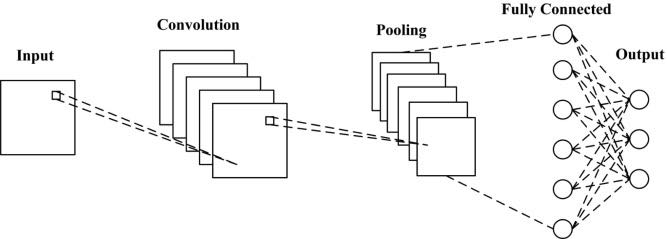
\includegraphics[width=0.47\textwidth]{CNN-model.jpg}
    \caption{CNN Model}
    \label{fig:cnn-model}
\end{figure}
\vspace{1em}

Convolutional Neural Networks (CNNs) (\autoref{fig:cnn-model}) are a powerful tool for extracting spatial
features from audio data. When audio is converted into spectrograms, which visually
represent sound, CNNs can identify local patterns like edges and textures in the data \cite{oshea2015introduction}.
One of the biggest advantages of CNNs is their translational invariance, which makes the
model resistant to shifts and distortions in the input data. Moreover, CNNs significantly
reduce the number of parameters by sharing weights, making the training process more
efficient. This model is also easily scalable by adding more layers and filters, allowing
for the extraction of increasingly complex features.

Research group proposed a CNN model begins with an input layer
designed to accept an input image. It first applies a 2D
convolutional layer with 32 filters, a 3x3 kernel size, and ReLU
activation, followed by a max pooling layer with a 2x2 pool size and
strides of 2x2 to downsample the feature maps. The process is repeated
with a second convolutional layer, this time with 64 filters and the
same kernel size and activation, followed by another max pooling layer
with identical parameters. The feature maps are then flattened into a
1D vector, which is passed through a series of fully connected (dense)
layers. The first dense layer has 64 units with ReLU activation,
followed by a second dense layer with 250 units and ReLU activation,
and a third dense layer with 100 units and ReLU activation. This model
concludes with an output dense layer containing a single unit with a
sigmoid activation function for binary classification tasks.

However, CNNs have some limitations. The model primarily captures spatial features and may
not be effective in capturing the temporal dependencies inherent in sequential
audio data \cite{lim2020time}. CNNs also require a fixed input size, which can be a limitation when
processing audio segments of varying lengths. Additionally, audio data needs to be
converted into spectrograms or other image-like representations before being fed into a CNN,
requiring an additional preprocessing step.

\vspace{-1em}
\begin{figure}[H]
    \centering
    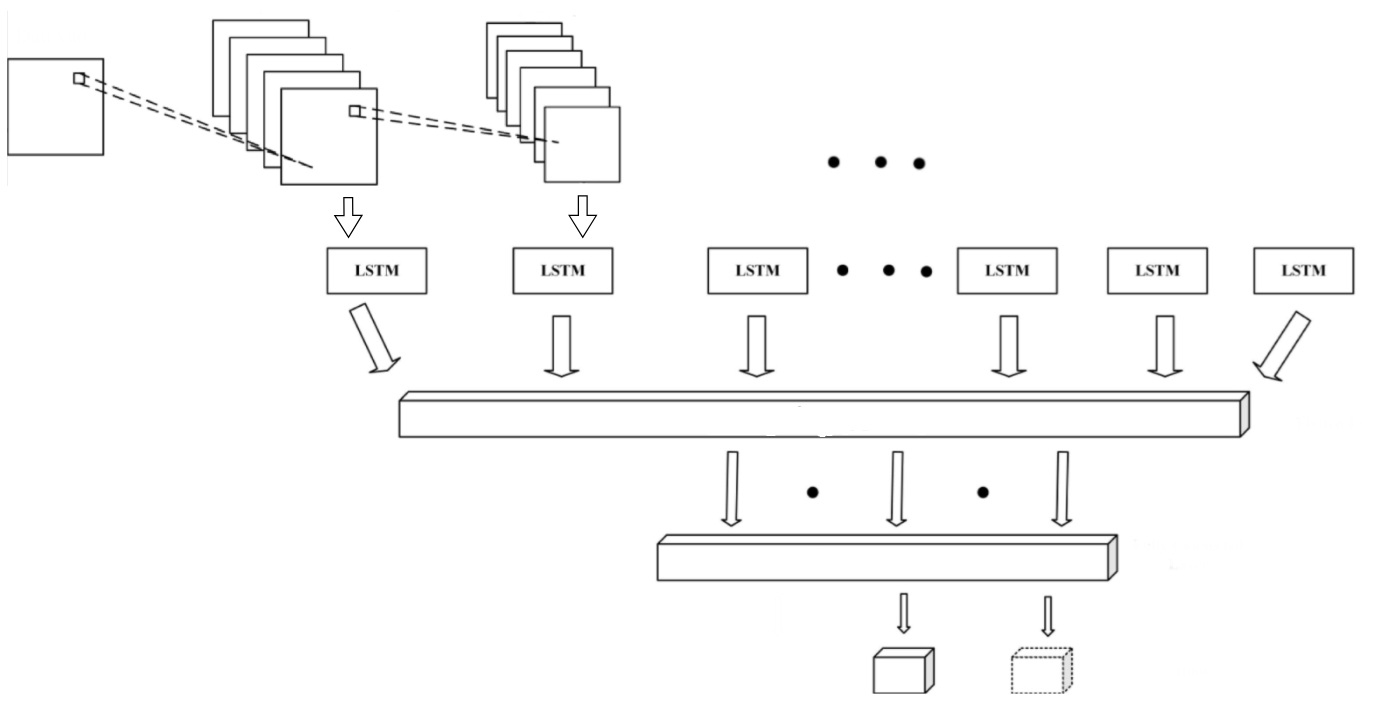
\includegraphics[width=0.47\textwidth]{LSTM-CNN-model.png}
    \caption{LSTM+CNN Model}
    \label{fig:lstm-cnn-model}
\end{figure}
\vspace{-1em}

In this study, we utilize a hybrid LSTM+CNN (\autoref{fig:lstm-cnn-model}) 
model to leverage the strengths of both architectures: the Convolutional Neural Network (CNN) 
for automatic feature extraction from spatial data and the Long Short-Term Memory (LSTM) 
network for capturing temporal dependencies in sequential data. This combined approach is 
designed to enhance model performance on tasks involving both spatial and temporal patterns. 
For a detailed explanation of the LSTM+CNN architecture and its implementation, please refer 
to the Appendix section.

In summary, we have outlined the advantages and disadvantages of our
models, CNN and LSTM+CNN, based on the theoretical foundation. The
evaluation of the performance of the two models, based on accuracy and
computational speed, will be conducted through practical experiments
on the bee audio dataset collected through IoT devices installed by
the group at the bee farm.
